\chapter{EMG and Nerve-Conduction Studies}

\section*{Overview}
Electromyography (EMG) and nerve-conduction studies (NCS) are tests of nerves and muscles. They are often done during the same appointment, but a person may need only one part. NCS uses small electrical pulses on the skin to measure how nerves carry signals. Needle EMG uses a fine needle electrode to record the electrical activity that muscles naturally produce. The tests do not send an electrical current through the needle into the muscle.


\begin{center}
\begin{minipage}{\textwidth}\centering
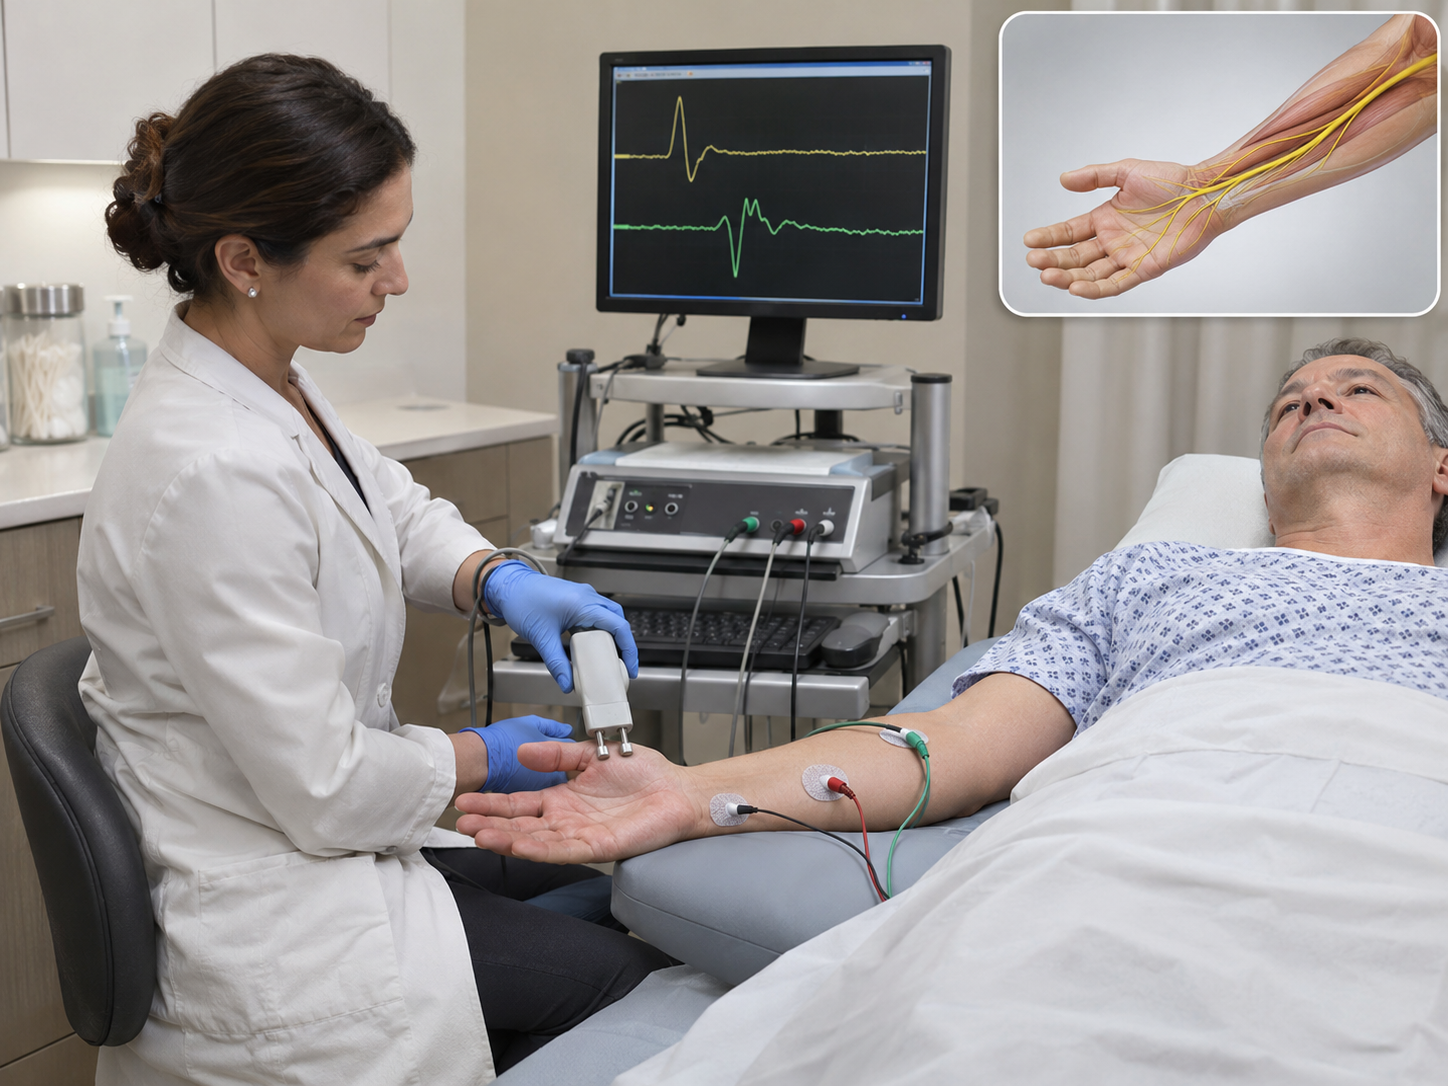
\includegraphics[width=0.82\textwidth]{images/chapters/procedure_electromyography_emg_overview.png}
\captionof{figure}{EMG and Nerve-Conduction Studies: A clinician tests muscle and nerve activity with electrodes and a recording unit.}
\end{minipage}
\end{center}
\section*{Common Instruments and Equipment}
The exact setup varies by technique and setting. Common items may include:
\begin{itemize}[nosep,leftmargin=*]
  \item EMG recording system and surface electrodes
  \item sterile needle electrodes for needle examination
  \item nerve-stimulation probe and cleaning supplies
\end{itemize}

\section*{Alternative Names}
Electrodiagnostic testing; nerve-conduction velocity study (NCV); needle EMG; NCS/EMG.

\section*{Principle}
NCS measures the size and timing of responses after a nerve is stimulated through the skin. Needle EMG records selected muscles while they are relaxed and when they tighten. These measurements can help identify whether symptoms are related to a nerve, nerve root, muscle, or, with specialized testing, the connection between nerve and muscle.

\section*{Why It Is Done}
The tests may help evaluate weakness, numbness, tingling, muscle cramps, or unexplained pain. They can help assess conditions such as nerve entrapment (for example, carpal tunnel syndrome), peripheral neuropathy, a pinched nerve root, or muscle disease. Specialized testing may be used for disorders of the neuromuscular junction. The tests are chosen based on the symptoms and examination.

\section*{Role in Care}
EMG and NCS are diagnostic tests. They can help locate and characterize a problem but do not always identify its cause. They do not test the brain or spinal cord directly, and results are considered along with the person's history, examination, imaging, and other tests. A normal result does not rule out every nerve or muscle disorder, especially if the condition is early, intermittent, or outside the nerves and muscles tested. After a recent nerve injury, the best timing depends on the suspected injury and the clinical question. An early study can still provide useful information, but repeat testing may sometimes be needed as changes develop.

\section*{How It Is Performed}
NCS is usually done first. The examiner places small recording electrodes on the skin and stimulates selected nerves with brief electrical pulses. The pulses may feel like a tap or brief shock and can make a muscle twitch. For needle EMG, a thin, sterile needle electrode is placed into selected muscles, one at a time. The examiner records activity while each muscle is relaxed and briefly tightened. The needle records natural muscle signals; it does not deliver the stimulus. The appointment often takes about 30 to 60 minutes, but it may be shorter or longer depending on which tests and how many areas are needed.

\section*{Preparation}
Wear loose clothing that allows access to the area being tested. Keep the skin clean and do not apply lotion, oil, or cream to it on the day of the test. Keep hands and feet warm if they are being examined, because cold can affect nerve measurements. Tell the examiner if you take blood thinners or aspirin, have a bleeding disorder, have a pacemaker or defibrillator, or have had surgery or other procedures in the area. Do not stop medicines unless your clinician specifically tells you to; anticoagulants and antiplatelet medicines are not routinely stopped for these tests.

\section*{Contraindications}
Pacemakers and defibrillators do not automatically prevent testing, but the examiner should know about them in advance. If you have myasthenia gravis or take medicines that affect muscle function, ask the testing team whether to take your usual dose before the appointment; do not change it without their advice.

\section*{Precautions}
Most people can have these tests. The clinician may adjust which muscles are tested or how the study is done based on bleeding risk, skin infection, recent surgery, implanted devices, or other health conditions.

\section*{Risks}
NCS can cause brief discomfort or tingling. Needle EMG may cause short-lived pain, muscle soreness, or a small bruise. Minor bleeding can occur at a needle site. Significant bleeding, infection, or other complications are rare. The examiner can pause or adjust the study if it becomes too uncomfortable.

\section*{Aftercare and Recovery}
Most people return to usual activities immediately. Muscles tested with a needle may feel sore for a short time, and small bruises can occur. Follow the testing team's advice and contact them if pain, swelling, or bruising is severe or getting worse.

\section*{Outcome and Follow-up}
The specialist reviews nerve response size and timing and the pattern of muscle activity. The report may help distinguish a nerve problem from a muscle problem and identify which nerves or muscles are affected. Results are usually sent to the clinician who requested the test, who will explain them with the rest of the evaluation. The study may not answer every clinical question, and additional testing may be needed.

\section*{Expected Results}
The study produces measurements and a report about the nerves and muscles tested. It does not give a complete picture of every nerve, muscle, or possible cause of symptoms.

\section*{Follow-up}
Discuss the report with the clinician who ordered the test. Further tests or treatment depend on the result and the person's symptoms. Ask the testing center when the report will be available.

\section*{When to Seek Medical Care}
Contact the testing team or a clinician for worsening pain, increasing swelling, persistent bleeding, or signs of infection at a needle site. Seek urgent care for severe or rapidly worsening symptoms.

\section*{References}
\begin{enumerate}
  \item MedlinePlus. Electromyography (EMG) and Nerve Conduction Studies. https://medlineplus.gov/lab-tests/electromyography-emg-and-nerve-conduction-studies/
  \item American Association of Neuromuscular \& Electrodiagnostic Medicine. FAQs Before EDX Testing. https://www.aanem.org/clinical-practice-resources/patient-information/faqs-before-edx-testing
  \item Cambridge University Hospitals NHS Foundation Trust. Nerve Conduction Studies and Electromyography. https://www.cuh.nhs.uk/patient-information/nerve-conduction-studies-ncs-and-electromyography-emg/
  \item American Association of Neuromuscular \& Electrodiagnostic Medicine. EMG/NCS and Risk of Bleeding. https://www.aanem.org/docs/default-source/documents/aanem/practice/emg-ncs-and-risk-of-bleeding.pdf
  \item American Association of Neuromuscular \& Electrodiagnostic Medicine. Recommended Policy for Electrodiagnostic Medicine. https://www.aanem.org/docs/default-source/documents/aanem/practice/recommended-policy-edx-medicine-062810.pdf
\end{enumerate}

\clearpage
